\documentclass[10pt]{article} % Font size - 10pt, 11pt or 12pt

\usepackage[hmargin=1.25cm, vmargin=1.5cm]{geometry} % Document margins

\usepackage{graphicx}
\usepackage{amsmath}
\usepackage{listings}

\usepackage[usenames,dvipsnames]{xcolor} % Allows the definition of hex colors

% Fonts and tweaks for XeLaTeX
\usepackage{fontspec,xltxtra,xunicode}
\defaultfontfeatures{Mapping=tex-text}
%\setmonofont[Scale=MatchLowercase]{Andale Mono}

% Colors for links, text and headings
\usepackage{hyperref}
\definecolor{linkcolor}{HTML}{506266} % Blue-gray color for links
\definecolor{shade}{HTML}{F5DD9D} % Peach color for the contact information box
\definecolor{text1}{HTML}{2b2b2b} % Main document font color, off-black
\definecolor{headings}{HTML}{701112} % Dark red color for headings
% Other color palettes: shade=B9D7D9 and linkcolor=A40000; shade=D4D7FE and linkcolor=FF0080

\hypersetup{colorlinks,breaklinks, urlcolor=linkcolor, linkcolor=linkcolor} % Set up links and colors

\usepackage{fancyhdr}
\pagestyle{fancy}
\fancyhf{}
% Headers and footers can be added with the \lhead{} \rhead{} \lfoot{} \rfoot{} commands
% Example footer:
%\rfoot{\color{headings} {\sffamily Last update: \today}. Typeset with Xe\LaTeX}

\renewcommand{\headrulewidth}{0pt} % Get rid of the default rule in the header

\usepackage{titlesec} % Allows creating custom \section's

\allowdisplaybreaks

% Format of the section titles
\titleformat{\section}{\color{headings}
\scshape\Large\raggedright}{}{0em}{}[\color{black}\titlerule]

\title{Bioinformatics Assignment 4}
\author{Elliott Capek}
\titlespacing{\section}{0pt}{0pt}{5pt} % Spacing around titles

\begin{document}

\maketitle{}

\section{Problem one: RNA duplexes}
We put the 5' and 3' microRNA sequences into a fasta file and use the command
\texttt{RNAduplex} to find their duplex energies. Example command:
\texttt{cat duplex.fa | RNAfold}\\

\textbf{hsa-let-7a: } $\Delta G = -23.50$\\
\textbf{hsa-mir-9: } $\Delta G = -23.00$\\
\textbf{hsa-let-7a: } $\Delta G = -15.50$\\

\section{Problem two: Inter-species RNA duplexes}
We put the 5' human RNA sequences and the 3' Drosophila sequence into a fasta file
and recomputed the duplex energies in the same way as in Problem One:\\
\textbf{dme-let-7: } $\Delta G = -20.4$\\
\textbf{dme-mir-9a: } $\Delta G = -17.3$\\
\textbf{dme-mir-100: } $\Delta G = -16.5$\\

As we can see, these duplexes are a higher energy than the human-human duplexes, which
is to be expected because DNA sequences drift over time, and divergences from the
original sequence are more likely to increase the duplex energy than decrease it.\\

\section{Problem three: RNA structure commands}
\textbf{a.)} \texttt{cat duplex.fasta | RNAduplex -T 26}\\
\textbf{b.)} \texttt{cat hotair.fasta | RNAfold -T 35}\\

\section{Problem four: }
Here we take a normal RNA sequence and compute its energy by using RNAduplex on it with
its reverse complement. We then take the sequence and concatenate it with its reverse
complement, and successively add ``CA'' non-bonding pairs to the center to form a
loop. We then use RNAfold on each length of the loop to find its energy. We then plot
these energies along with the $1.75*RT*ln(l)$, the theoretical energy, to see how
well the relationship holds.\\

\begin{figure}[h!]
  \caption{}
  \centering
  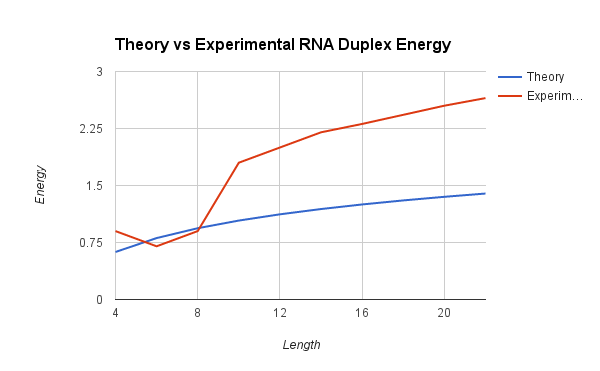
\includegraphics[width=0.5\textwidth]{../duplex_energy.png}
\end{figure}

From this figure we can see that the trend is mostly logarithmic, except there is a
slight dip in energy at loops of length 6 and 8. This is weird. This could be due to
a geometry thing - perhaps loops of this size are stabilized due to orbitals aligning,
like the plot of cycloalkane stability with length.\\

\section{Problem five: RNA duplex free energy}
Here we take 40-length AU or GC sequences and compute their duplex energy with their
reverse complements. We calculate an energy of -108.28 kcal/mol for 40 C-G alternating
bonds and -41.8 kcal/mol for 40 A-U alternating bonds. We divide by 40 to get -2.7
kcal/mol for a C-G bond (assuming neighbors of C-G bonds, value will be different
for different neighbors) and -1.045 kcal/mol for A-U bonds.\\

\section{Problem six: TopHat command}
Here we use the following command to align reads\_rep1.fastq to the mm10 mouse genome
index, using the mouseGenes.gtf annotation file:\\

\texttt{tophat -o reads\_mm10\_tophat
  -G mouseGenes.gtf mm10 reads\_rep1.fastq}

\section{Problem seven: Cuffdiff}
RPKM stands for \textbf{Reads per Kilobase} of gene per length per \textbf{Million}.
This is basically taking the number of reads mapped to a gene over the total number
of reads, which is the ``activity'' of that gene. This number then needs to be corrected
for the length of the transcript, so we divide by the transcript length.\\

FPKM stands for \textbf{Fragments per Kilobase} of gene per length per \textbf{Million}.
This is the exact same as RPKM, except fragments of cDNA are used instead of just reads.
Fragments are better because they take into account things like paired-end effects.\\

\section{Problem eight: Cuffdiff options}

\textbf{a.)} The \texttt{-L/--labels} option can be used to specify the labels used
in the \texttt{cuffdiff} output. This is a comma-separated lsit if multiple labels
are to be used.\\

\textbf{b.)} \texttt{cuffdiff} finds expression levels for transcripts, it doesn't create
a map of transcripts, or transcriptome. \texttt{cufflinks} is the tool to create a
transcriptome assembly.\\

\section{Problem nine: Intersection vs Union}
Here we use the tutorial described in Trapnell 2013 to compute the log fold-change.\\

To compute via the union method, we just count the number of hits over the union of
the exons. We find that there are 25 hits for both Condition A and Condition B, so:

\begin{align*}
  \log_2\left(\frac{25}{25}\right) &= 0\\
\end{align*}

To find via the intersection method, we do the same with the intersection of the two
exons and find there are 19 hits for both Condition A and Condition B, so:

\begin{align*}
  \log_2\left(\frac{19}{19}\right) &= 0\\
\end{align*}

Finally to find the true expression, we count the hits for each exon they belong to
and divide by the exon's length:

\begin{align*}
  \log_2\left(\frac{\frac{14}{3L}+\frac{11}{2L}}{\frac{15}{3L}+\frac{9}{2L}}\right)
  &= \log_2\left(\frac{\frac{28+33}{6L}}{\frac{30+27}{6L}}\right)\\
  &= \log_2\left(\frac{61}{57}\right)\\
  &= 0.098\\
\end{align*}

\end{document}
